\chapter{Preparation of Approach}
\label{ch:PrepApproach}
This chapter provides fundamental information about the techniques and notation used in the approach. As introduced in Chapter \ref{ch:CoCoME}, the Case Study's system specification is given in terms of detailed use cases. However, the proposed approach uses business processes as input. It is therefore necessary to provide a formal concept that assists with transforming use cases into business processes. \\
The following sections introduce a well known and established use case notation technique, a standardized notation to capture business processes and a structured approach to transform use case sets as business processes. Further, the extraction of data flow and control flow from business processes is discussed.


\section{Use Cases}
\label{sec:PrepApproach:UC}
Use Cases are a widely adopted technique to document software system requirements. Generally, they describe the interaction between actors (usually system users) and the software system itself. In this thesis, use cases are provided as semi-structured tables (following the notation presented by Cockburn et al. \cite{Cockburn}). \\ An example is given in Table \ref{tab:exampleUseCase}: Each use case has a unique identifier and a short description, followed by necessary preconditions and a trigger that causes the execution. The standard process is the main part and describes the success steps of the Use Case. Extensions provide additional information like alternatives or exceptional processes that occur in case of an unsuccessful step. 




\begin{table}[!h]
	\centering
	\begin{tabularx}{\textwidth}{|l||X|}
		\hline
	    UC 5 & Show Stock Reports \\ 
	    \hline
	    Brief Description &  The opportunity to generate stock-related reports is provided
	    by the Trading System. \\
	    \hline
	    Precondition & The reporting GUI at the Store Client has been started. \\
	    \hline
	    Trigger & The Store Manager wants to see statistics about his store. \\
	    \hline
	    Postcondition & The report for the Store has been generated and is displayed on
	    the reporting GUI. \\
	    \hline 
	    Standard Process &
	       
	            1. The Store Manager enters the store identifier and presses the button Create
	                     Report.  \\
	           & 2. A report including all available stock items in the store is displayed. \\  
        \hline
        Extensions & (none) \\ \hline
	   
		
	\end{tabularx}
	\caption{Example Use Case in Tabular Form, Source: \cite{CoCoMEOld}}
	\label{tab:exampleUseCase}
	
\end{table}

\noindent
The usage of Use Cases as input for the approach has a remarkable benefit: Besides being a widely adopted technique to specify system requirements, the textual use case notation is understandable without further technical knowledge. Neither previous knowledge in specific graphic notations like UML, nor the capability to create a complex domain model is necessary. Consequently, all sort of stakeholders (non-technical and technically experienced) are capable to provide the necessary information in terms of use cases. \\
However, the transformation as presented in Sec.\ref{sec:PrepApproach:TransformUCtoBPMN} is not always trivial and requires some manual effort to produce high quality business processes. 





\section{Business Process and Model Notation}
\label{sec:PrepApproach:BPMN}
The Business Process and Model Notation (BPMN) is a graph oriented language to describe business processes. Originally, BPMN was designed to describe activities and their control flow dependencies only \cite{VisualizeBPMN}. Since the introduction of BPMN 2.0, it is possible to model the data needs and the data results of activities \cite{OMG}. Consequently, BPMN is capable to express the control flow and data flow of business processes \cite{DataFlowErrorBPMN}. In the remainder, we use BPMN instead of BPMN 2.0 for the sake of convenience. \\
BPMN is easy-to-use, powerful and widely adopted in academia and industry. Hence, BPMN is a suitable approach to extract the implicitly given data flow and control flow in the use case description. Sec. \ref{sec:Fundamentals:TransformUCtoBPMN} introduces a formal approach to generate BPMN processes from use case sets. Next, the BPMN 2.0 process definition is shortly introduced:


\begin{figure}[h!]
	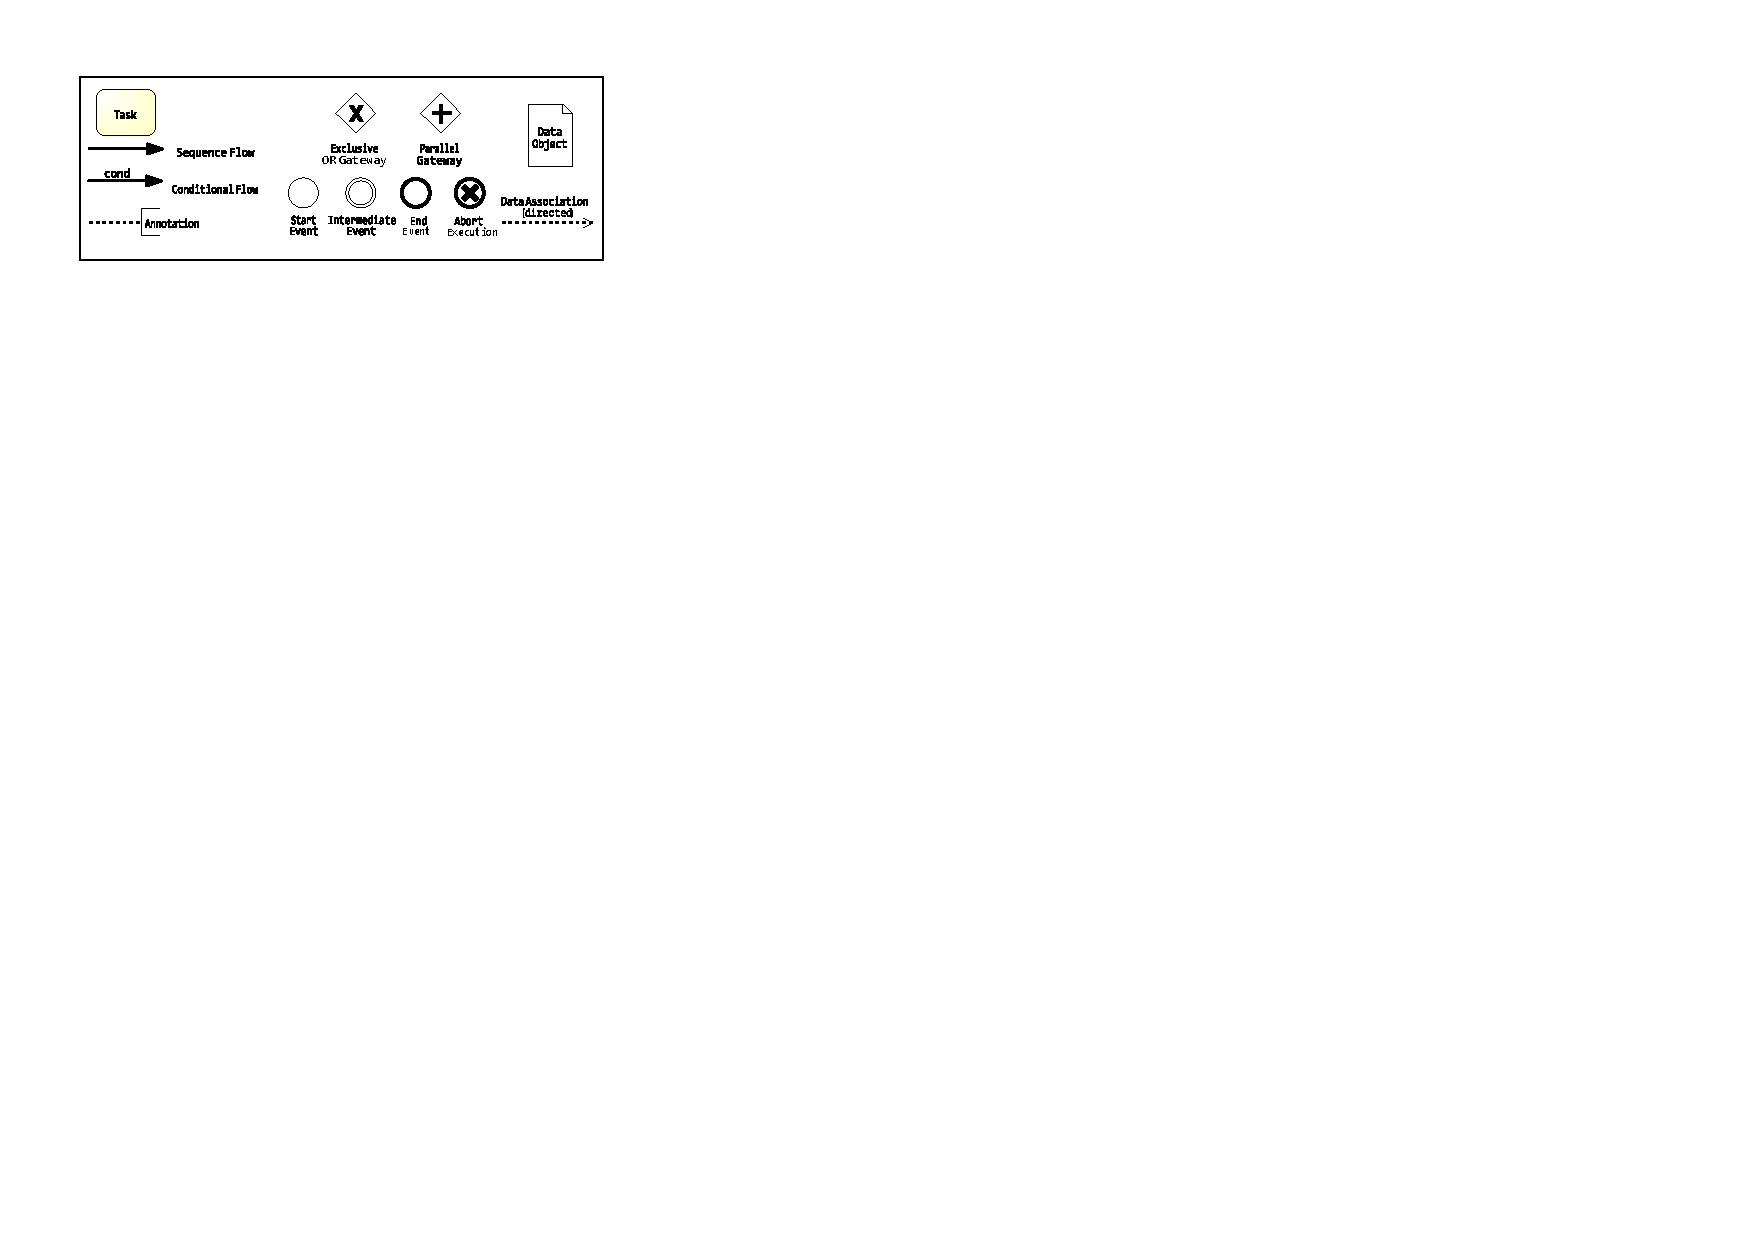
\includegraphics[width=\textwidth, trim={1cm 16.5cm 19.2cm 1cm}]{img/Overview.pdf}
	\caption{BPMN Notation (Subset)}
	\label{fig:BPMNSubset}
\end{figure}

\noindent
Fig.\ref{fig:BPMNSubset} presents the subset of BPMN symbols, that is required for the approach presented in this thesis \footnote{The entire specification is available at https://www.omg.org/spec/BPMN/2.0/}. Control flow activities are modelled as atomic \textit{Tasks} and connected through \textit{Sequence Flow Arcs}. \textit{Conditional Flow Arcs} integrate decision points into the control flow. Navigation decisions are based on the conditions related to the individual arcs. Such decision point are the \textit{Exclusive Or Gateway} and the \textit{Parallel Gateway}. Regarding the first one, if one of the incoming flows is triggered exactly one outgoing flow is activated based on the condition. For the latter, all outgoing flows are activated as soon as all of its incoming flows are activated. Each BPMN process starts with a \textit{Start Event} and ends with an \textit{End Event}. In case of several branches (due to Gateways), stop events need to be placed to each end. \textit{Intermediate Events} mark any other events that occur during the process. The trigger for an event is modelled using the \textit{Annotation} symbol. \textit{Abort Execution Event} extend the \textit{End Event} and marks the error-prone end of a business process. \\
When it comes to data, each \textit{Task} may or may not require and/or produce data. Directed \textit{Data Association Arcs} provide the opportunity to model the data flow. In case a task requires data, the corresponding \textit{Data Objects} are connected to the task with the arrowhead attached to the task. Producing data works in the opposite direction. \\









\section{Use Case Sets and BPMN Processes}
\label{sec:PrepApproach:TransformUCtoBPMN}
To visualize the implicit data and control flow in use cases, it is necessary to transform the given use cases into BPMN models. In "Visualizing Use Case Sets as BPMN Processes" \cite{VisualizeBPMN}, Lübke et al. already elaborated an approach to visualize the control flow that is hidden in use cases. As Lübke does not use the BPMN 2.0 notation, data is not considered and hence, data flow is not part of the given approach. In the following, we will introduce a conceptional approach, which is based on \cite{VisualizeBPMN}, to transform use cases into BPMN models and extract the data flow and control flow.


\subsection{Transform Use Case Sets in BPMN Processes}
To visualize use case sets, including data flow and control flow, the following elementary steps need to be performed:

\begin{enumerate}
	\item Create a flat use case model. Replace \textit{include} and \textit{extend} relationships by the associated use case
	\item Generate an independent BPMN process for each use case
    \item Join the generated BPMN processes based on preconditions, trigger and postconditions
    \item Remove duplicate Data Objects and refactor the data associations
    \item Refactor the business model i.e. divide or remove unnecessary steps, identify synonymous data objects, trigger etc.
\end{enumerate}


\begin{figure}[h!]
	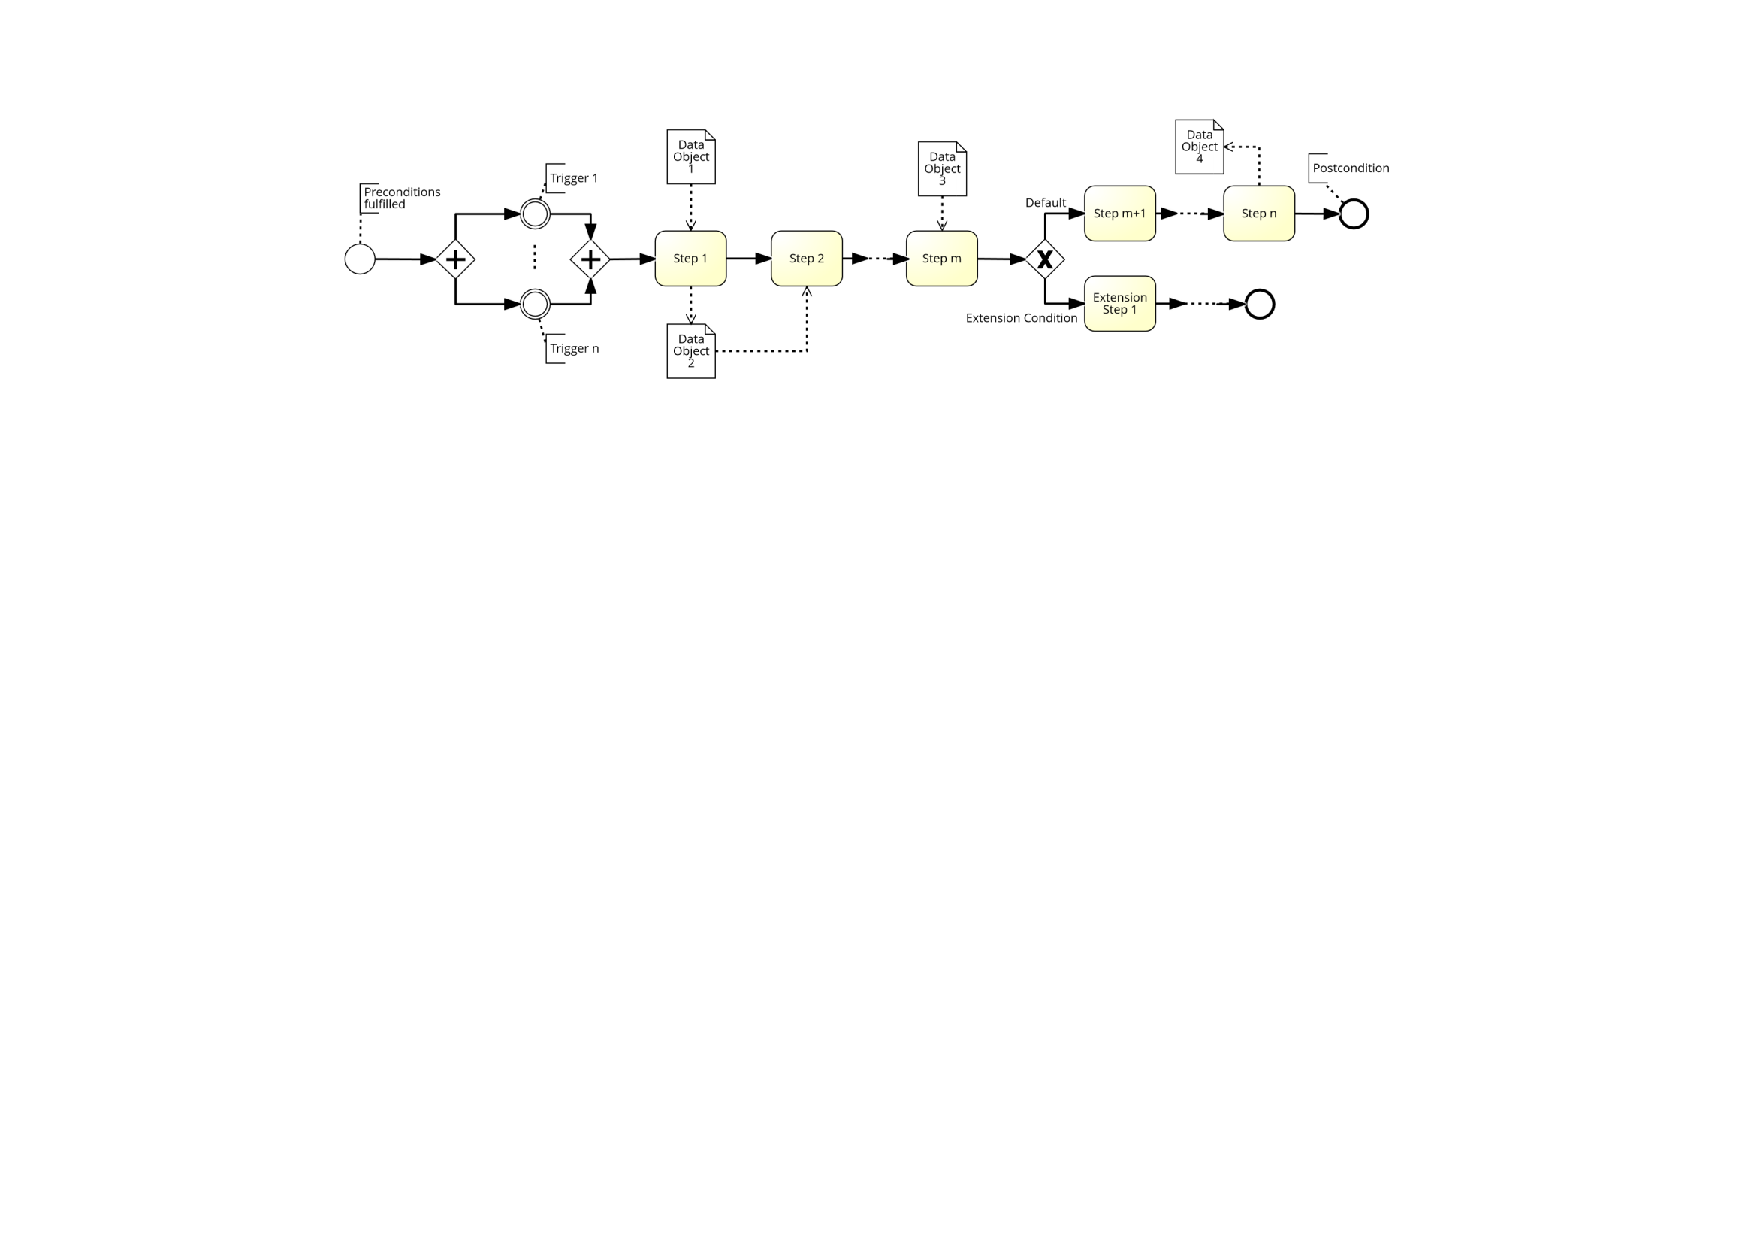
\includegraphics[width=\textwidth, trim={6cm 14.5cm 6cm 1.5cm}]{img/usecaseTransformation.pdf}
	\caption{Use Case transformed in a BPMN process}
	\label{fig:useCaseTransformation}
\end{figure}
The first step only includes simple substitutions, as the \textit{extend} and \textit{include} relationships simply have to be replaced by the actual use case.\\
Step number two represents the main part of the transformation. Fig.\ref{fig:useCaseTransformation} is an additional illustrative diagram that explains this step. First, the preconditions is assigned to the start event by using an annotation. Triggers are represented by intermediate events and as they are executed in parallel, connected by two Parallel Gateways. Each step in the use cases standard process is represented by a single task. This procedure might include some refactoring as further enlightened in the final step. Tasks that produce and/or consume data are connected to the corresponding data object. It has to be noticed, that data objects appear only once in a model. Given these point, it is necessary to check if a data object is already referenced by a previous task. Jumps and alternatives are modelled using Exclusive Or Gateways. Finally, the postcondition is added as annotation and connected to the end event. \\
Joining the use case-based BPMN models is necessary to represent the control flow and data flow within the entire system. (The flows are generally not limited to "use case borders"). For each pair of use cases (\textit{UC A} and \textit{UC B}), check if the postcondition of UC A exists as precondition or trigger of UC B. If this is the case, join the accompanying BPMN processes by deleting the start event (BPMN process of UC B) and the end event (BPMN process of UC B) and connect the graphs. In case that multiple use cases have the same postcondition, their BPMN processes are connected using an Exclusive Or Gateway (Fig.\ref{fig:JoinBPMNPostcondition}). If several use cases have the same preconditions or triggers and therefore use the same postcondition (Fig.\ref{fig:JoinBPMNPrecondition}), join them by introducing a Parallel Gateway and split the control flow. Notice, that the use cases in Fig.\ref{fig:JoinBPMNPostcondition} and Fig.\ref{fig:JoinBPMNPrecondition} are only displayed as collapsed subprocess for the sake of clarity. 

\begin{figure}[h!]
	\centering
	\begin{minipage}{0.45\textwidth}
		\centering
		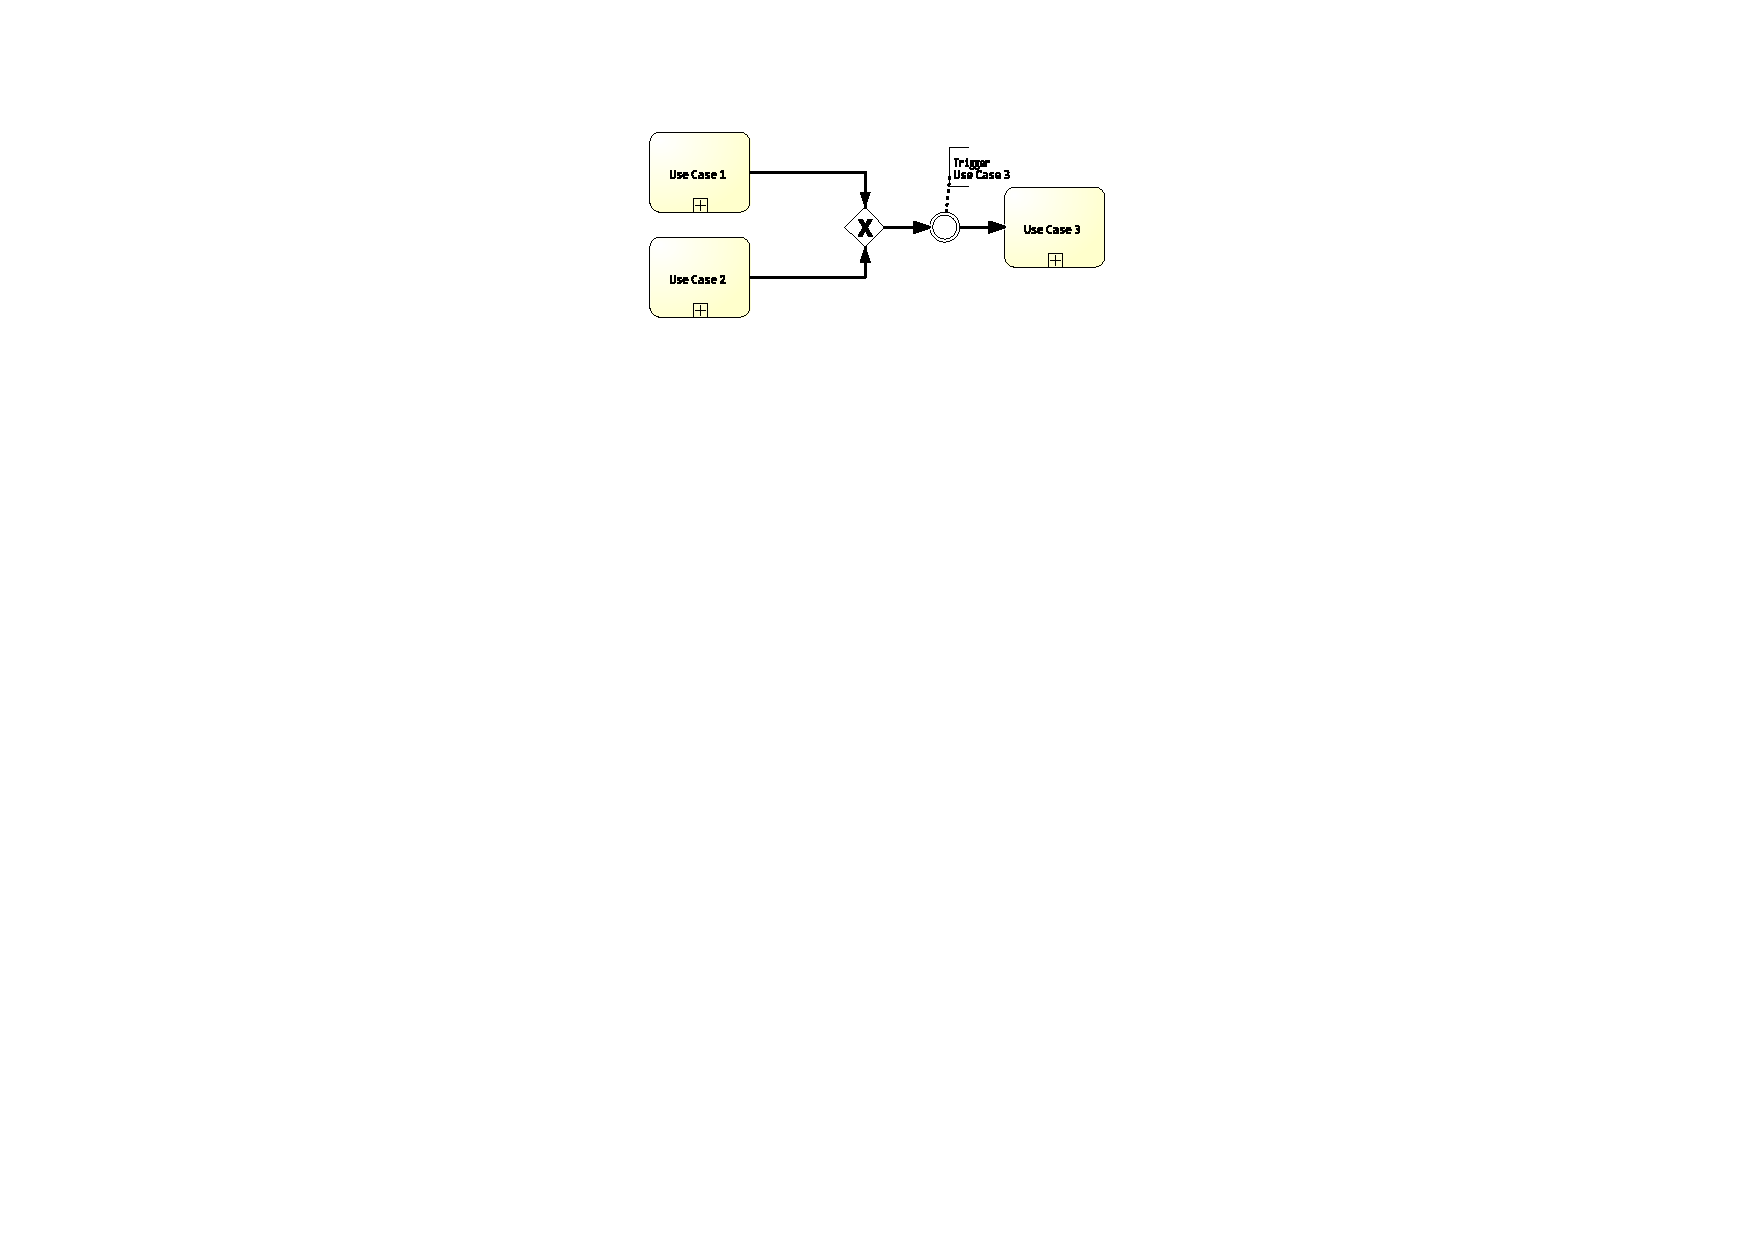
\includegraphics[width=0.9\textwidth, trim={11cm 15cm 12cm 1cm}]{img/JoinBPMNpostcondition.pdf} % first figure itself
		\caption{Join BPMN processes on same postconditions}
		\label{fig:JoinBPMNPostcondition} %11cm 14cm 18cm 1cm
	\end{minipage}\hfill
	\begin{minipage}{0.45\textwidth}
		\centering
		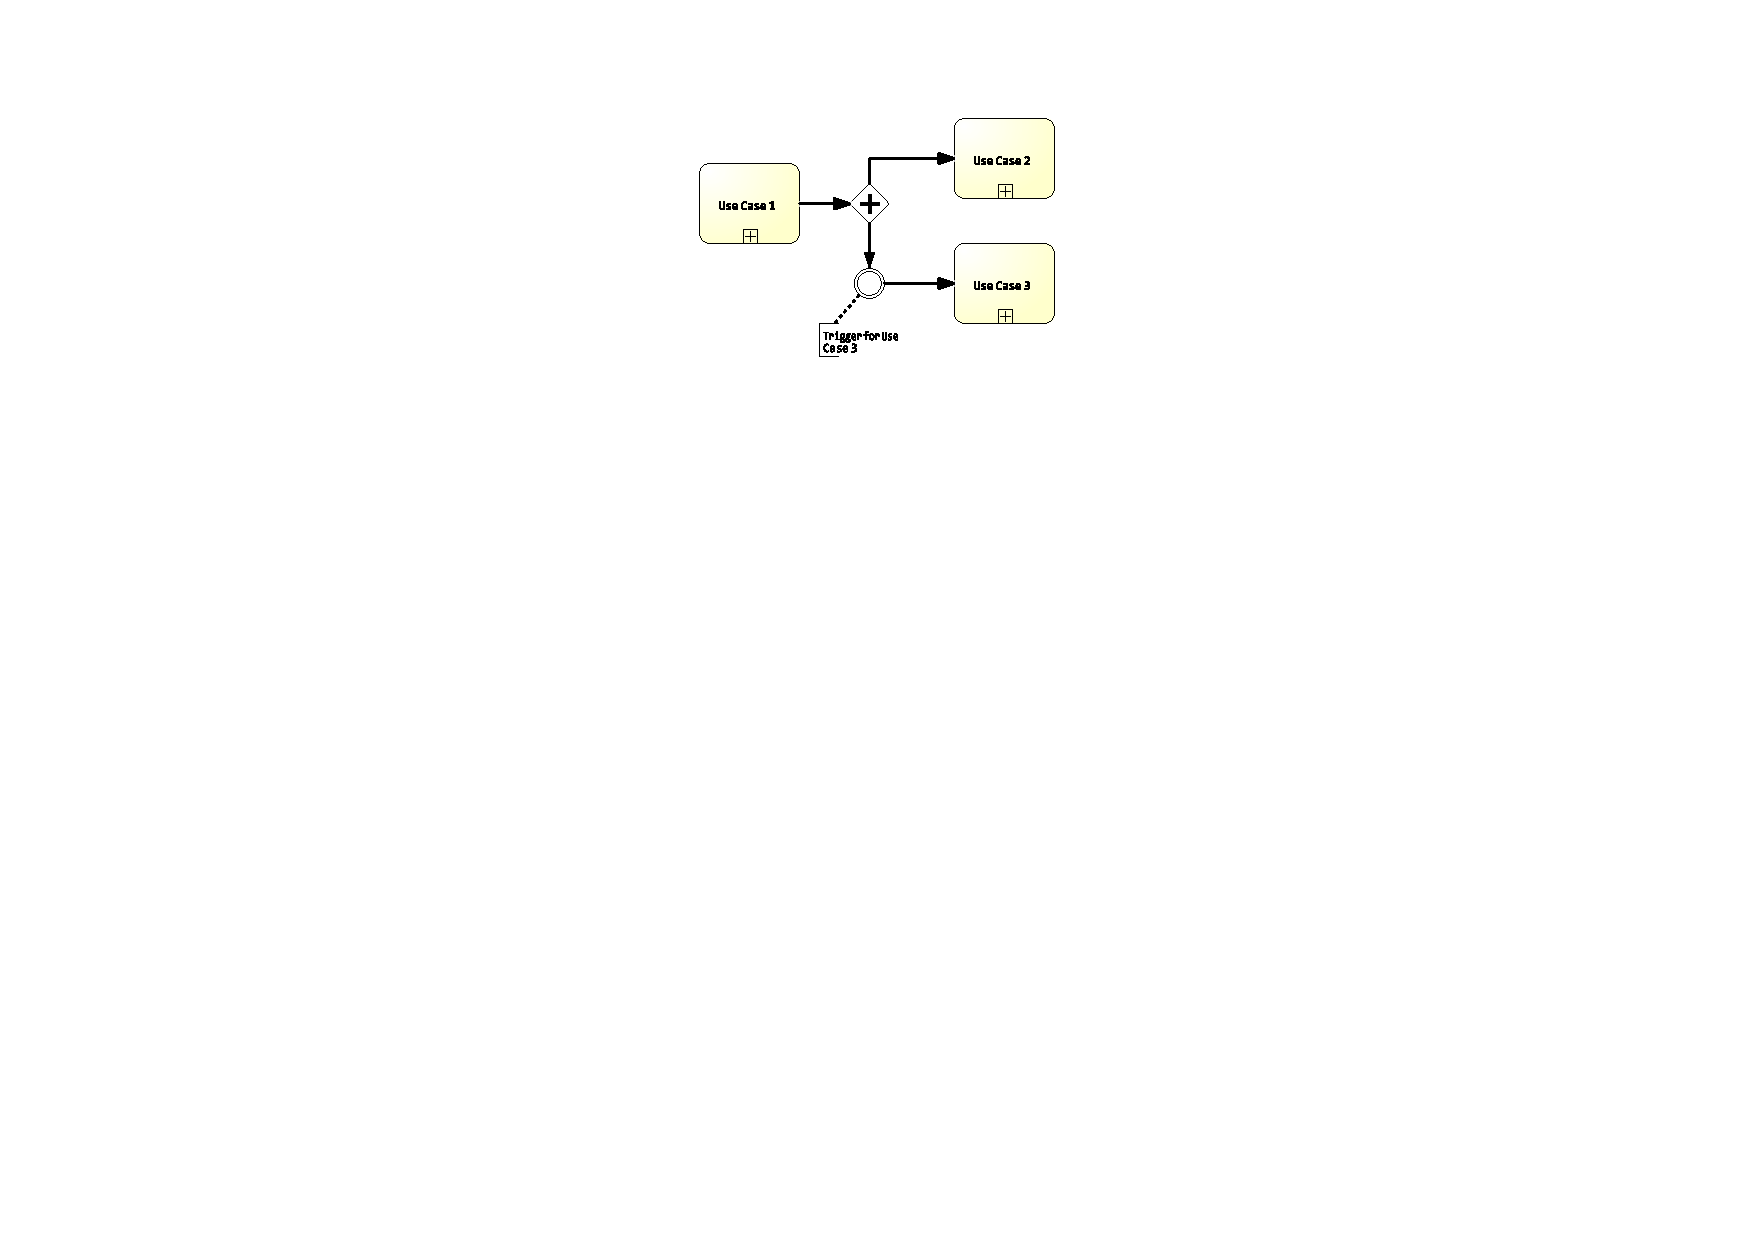
\includegraphics[width=0.9\textwidth, trim={11cm 15cm 12cm 1cm}]{img/JoinBPMNPrecondition} % second figure itself
		\caption{Join BPMN processes on same preconditions or triggers}
		\label{fig:JoinBPMNPrecondition}
	\end{minipage}
\end{figure}

Second to last, the resulting data associations and objects are refactored. Duplicate Data Objects that arose from joining two processes need to be eliminated. For each set of duplicate data objects, remove all but one and reconnect the existing Data Associations to the remaining object. \\
Finally, the entire business models need to be refactored. Whereas the prior steps are very algorithmic and follow a predefined concept, this step includes non-trivial work. Due to the fact that use cases are given in natural language, one has to identify synonymous data objects,steps, triggers, post- and preconditions. Moreover, a step in an use case may include two activities and has to be split up.
For example, given these two steps from two different use cases:
\begin{itemize}
	\item \textit{The Store Manager changes the sales price of the Stock Item and commits the change by pressing enter}
	\item \textit{The sale information is sent to the Inventory in order to update the Stock}
\end{itemize}
Both steps update the same Data Object, which is the Stock Item, although the second step refers to the object as \textit{Stock}. The activity in both cases can be described as \textit{Update inventory}. Furthermore, steps one contains two activities and needs to be split in \textit{Change Price} and \textit{Update Inventory}.

\subsection{Limitations and Drawbacks of the Transformation}
In Chapter \ref{ch:Solution}, we present an approach that identifies microservices from the business point of view using BPMN processes as input. Nevertheless, the case study we use only provides system specification in form of detailed use cases. Therefore, the previous sections present a transformation of use cases in a set of BPMN models. However, this transformation requires a non-trivial refactoring process. In regard to data objects, it is obvious that multiple appearances of the same object (in different shaping) in a process devastate the resulting data flow. Speaking of tasks, it is necessary to examine the impact on the clustering presented in Chapter \ref{ch:Solution}: It is indispensable to identify common tasks among all use cases and consequently the resulting business processes to create the structural relationship between them. If not, the tasks would be arranged in a circle-like order and the resulting clusters would correspond to the business processes. \\
For this reasons, the refactoring process has to be conducted 
conscientiously. If this is not the case or synonyms etc. are not identified, the results of the approach might not be satisfactory.


%TODO Nochmal drüber lesen


\section{Control Flow and Data Flow in BPMN Processes}
\label{ch:PrepApproach:ControlDataFlowBPMNProcess}

\subsection{Extract Control Flow of BPMN Processes}
Extracting the Control Flow in BPMN processes is a trivial task. The BPMN was originally designed to describe the control flow in business process. All that has to be done is to delete the Data Objects and the accompanying associations. The remaining diagram visualizes the control flow, including activities and their control flow dependencies. Further information, can be extracted in various ways. For instance, counting the amount of tasks between a pair of activities provides information about their structural dependency.

\subsection{Extract Data Flow of BPMN Processes}
%TODO Add DFD or BPMN Data Flow?

\subsection{Running Example}


Subprocess!



\textit{Example 1.} Fig . prese








